\documentclass{article}

\usepackage{amsmath}
\usepackage{graphicx}

\graphicspath{ {./assets/} }

\setlength\paperwidth{20.999cm}\setlength\paperheight{29.699cm}\setlength\voffset{-1in}\setlength\hoffset{-1in}\setlength\topmargin{1.499cm}\setlength\headheight{12pt}\setlength\headsep{0cm}\setlength\footskip{1.131cm}\setlength\textheight{25cm}\setlength\oddsidemargin{2.499cm}\setlength\textwidth{15.999cm}

\begin{document}
\begin{center}
\hrule

\vspace{.4cm}
{\bf {\Huge Assignment 2}} \\
\vspace{.2cm}
{\bf Computer Graphics}
\vspace{.2cm}
\end{center}
{\bf Edoardo Riggio } (edoardo.riggio@usi.ch) \hspace{\fill}  \today \\
\hrule
\vspace{.2cm}

\section*{Exercise 2}
In order to demonstrate that $\gamma = \frac{\beta}{2}$ we analyze three possible cases.

\subsection*{Case 1}
In this case we have that $d$ is after $c$, as shown in this image. \\
\begin{center}
  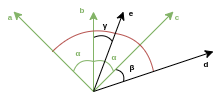
\includegraphics{./diagram_1.png}
\end{center}
In this case we have that the two angles in red (the one between $a$ and $e$, and the one between $e$ and $d$) are the same. This is because $e$ is the half-way vector between $a$ and $d$. Now we can see that:
\begin{align*}
  \alpha + \gamma & = \alpha + \beta - \gamma \\
  \alpha - \alpha + \gamma + \gamma & = \beta \\
  2 \cdot \gamma & = \beta \\
  \gamma & = \displaystyle\frac{\beta}{2}
\end{align*}

\subsection*{Case 2}
In this case we have that $d$ is between $b$ and $c$, as shown in this image. \\
\begin{center}
  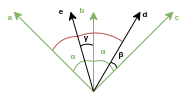
\includegraphics{./diagram_2.png}
\end{center}
In this case we have that the two angles in red (the one between $a$ and $e$, and the one between $e$ and $d$) are the same. This is because $e$ is the half-way vector between $a$ and $d$. Now we can see that:
\begin{align*}
  \alpha - \gamma & = \alpha - \beta + \gamma \\
  \alpha - \alpha - \gamma - \gamma & = - \beta \\
  -2 \cdot \gamma & = - \beta \\
  2 \cdot \gamma & = \beta \\
  \gamma & = \displaystyle\frac{\beta}{2} 
\end{align*}

\subsection*{Case 3}
In this case we have that $d$ is between $a$ and $b$, as shown in this image. \\
\begin{center}
  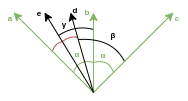
\includegraphics{./diagram_3.png}
\end{center}
In this case we have that the two angles in red (the one between $a$ and $e$, and the one between $e$ and $d$) are the same. This is because $e$ is the half-way vector between $a$ and $d$. Now we can see that:
\begin{align*}
  \alpha - \gamma & = \gamma - (\beta - \alpha) \\
  \alpha - \gamma & = \gamma - \beta + \alpha \\
  \alpha - \alpha - \gamma - \gamma & = - \beta \\
  - 2 \cdot \gamma & = - \beta \\
  2 \cdot \gamma & = \beta \\
  \gamma & = \displaystyle\frac{\beta}{2}
\end{align*}

\end{document}